\chapter{Empirische Verteilungen}
Es handelt sich hier überwiegend um die Bearbeitung von größeren gesammelten Datenmengen, wie man sie ordnet, wie man sie darstellt und wie man sie in Tabellen oder gar Kennzahlen zusammen fassen kann.
Ganz allgemein entstehen diese Daten durch Stichprobenerhebung oder Befragung. Wie die Erhebung oder Befragung organisier wird, ist Sache von Marktforschungsabteilungen.
\clm{Zusammenhang Datenerhebung und Datenqualität}{}{Man muss sich darüber im Klaren sein, dass die Daten niemals besser sein können, als die Erhebungsmethode, aus welcher sie hervorgingen.}
Daraus ergibt sich, dass Marktforscher im Idealfall gute Statistikkenntnisse aufweisen. Diese Vorlesung arbeitet jedoch nach dem Leitsatz: \textit{Statistik beginnt erst, wenn die Daten vorliegen!}

\section{Entstehung der Daten}
Man muss sich in diesem Rahmen
\begin{enumerate}
    \item zuerst darüber im Klaren sein, welche Frage eigentlich beantwortet werden muss. (\textbf{Forschungshypothese})
    \item dan Gedanken darüber machen, wie diese Frage beantwortet werden kann. Die Entstehung der \textbf{Untersuchungsvariablen}
\end{enumerate}
Um über die Qualität der Operationalisierung bzw der Messung urteilen zu können, müssen Gütekriterien her:
\begin{enumerate}
    \item \textbf{Objektivität:} Merkmalsauswahl bzw deren Auswerten und Interpretation sollte unabhängig vom jeweiligen Forscher erfolgen
    \item \textbf{Zuverlässigkeit:} Wird die Messung wiederholt, sollten ähnliche Ergebnisse rauskommen
    \item \textbf{Gültigkeit:} Messfehler sollten so klein wie möglich sein
\end{enumerate}

\section{Merkmale und ihre Eigenschaften}
Die empirische Statistik untersucht die Verteilung von Merkmalen oder Variablen, die nicht vorher durch Theorien bekannt sein können.
Die Ergebnisse sind nicht vorhersehbar, da das gemessene unter den Merkmalsträgern variiert.
\newline
Merkmale können als \textbf{Untersuchungsgegenstand} definiert werden. Es ist eine Eigenschaft, die an einem Untersuchungssubjekt (\textbf{Merkmalsträger}) beobachtet wird.
Die Merkmale und ihre \textbf{Merkmalsausprägungen} werden in der Planung der Untersuchung festgelegt.
\ex{Merkmalsträger und -ausprägung}{Bei einer Umfrage sind die befragten Personen die Merkmalsträger. Die abgefragten Gegenstände (Haarfarbe, Kinderzahl, Alter, Geschlecht) sind die Merkmale. Die Ausprägungen sind entsprechend (blond, schwarz, rot,..) und (0,1,2,..) usw.}

Wie man sieht, können sehr verschiedene Eigenschaften gemessen werden. Eine Untersuchung kann nur eine begrenzte Anzahl von Merkmalen aufnehmen und kann demnach nur als vereinfachtes Abbild der Realität fungieren.
\newline
Bei dem obigen Beispiel sind die Merkmale bewusst so gewählt worden. Es zeigt, dass die Ausprägungen sehr verschiedener Art sein können.
Diese Unterscheidung wird unter dem Begriff \textbf{Messniveau} zusammengefasst:
\dfn{Messniveaus / Skalierungen}{
Es wird in unterschiedliche Skalierungen unterteilt:
\begin{itemize}
    \item \textbf{qualitativ} (nicht-metrische Skalierung)
    \item \textbf{quantitativ} (metrische Skalierung)
\end{itemize}
Die nicht-metrische Skalierung wird wie folgt unterschieden:
\begin{itemize}
    \item \textbf{nominal}: Die Ausprägungen werden lediglich kategorisiert, ohne den Kategorien eine Rangfolge oder einen numerischen Wert zuzuweisen. (Geschlecht, Haarfarbe, etc)
    \item \textbf{ordinal}: Die Ausprägungen haben eine Rangordnung, allerdings ist der Abstand zwischen den Ausprägungen nicht gleichmäßig oder gar unbekannt. (Schulnoten (1, 2, 3, 4, 5, 6), Zufriedenheitsstufen (sehr zufrieden, zufrieden, unzufrieden, sehr unzufrieden) oder sozioökonomischer Status (niedrig, mittel, hoch))
\end{itemize}
Auf nicht-metrischen Skalen sind arithmetische Operationen nicht sinnvoll und teilweise auch nicht möglich.
Die metrische Skalierung wird wie folgt unterschieden:
\begin{itemize}
    \item \textbf{Intervallskala}: Die Ausprägungen haben eine Rangordnung und einen bekannten, gleichmäßigen Abstand. Es gibt jedoch keinen absoluten Nullpunkt. (IQ-Wert, Temperatur in Celsius)
    \item \textbf{Verhältnisskala}: Die Ausprägungen haben eine Rangordnung und einen bekannten, gleichmäßigen Abstand \textbf{und} einen absoluten Nullpunkt. Zusätzlich wird hier in \textbf{diskret} und \textbf{stetig} unterschieden.
\end{itemize}
Auf metrischen Skalen sind arithmetische Operationen sinnvoll.
Ist kein Nullpunkt vorhanden, so sind lediglich Addition und Subtraktion sinnig.
Ist ein Nullpunkt vorhanden, so können die Operationen um Multiplikation und Division ergänzt werden.
}
\nt{Bei Untersuchungen wird man oft feststellen, dass ein diskretes Mekrmal, welches sehr viele Ausprägungen (Geldbeträge in Cent) annehmen kann, häufig als stetiges Merkmal behandelt wird. Man spricht bei ihnen von \textbf{quasistetigen} Merkmalen. Andererseits werden auch einige stetige Merkmale als diskret erhoben (Lebensdauer).}

\section{Definition und Notationen}
\dfn{Grundbegriffe}{Die Menge aller für die Untersuchung relevanten Merkmalsträger ist die \textbf{Grundgesamheit}. \newline
Die Menge der in der Untersuchung betrachteten Merkmalsträger nennt man die \textbf{Strichprobe}. \newline
Die Gesamtheit aller Daten über Merkmale, Merkmalsträger und Merkmalsausprägungen wird als Beobachtungsdaten oder \textbf{Urliste} bezeichnet.
}
Man spricht immer von $n$ vorhandenen Merkmalsträgern. Es wird ein \textbf{Laufindex} $j$ für den j-ten Merkmalsträger definiert:
\[j=1,2,\dots,n-1,n\]
$X$ und $Y$ werden immer die Merkmale allgemein bezeichnen.
$x_j$ bezeichnet die Ausprägung von Merkmal $X$ für den j-ten Merkmalsträger.
\newline
Eine Datenreihe für ein Merkmal $X$ lautet dann entsprechend:
\[x_1, x_2, \dots, x_{n-1}, x_n\]

\section{Univariate Darstellung für verschiedene Merkmalsniveaus}
\subsection{Nominalskalierte Merkmale}
Nominalskalierte Merkmale lassen sich in einer Häufigkeitstabelle (\ref{fig:haeufigkeitstabelle-nominale-merkmale}) darstellen und zusammenfassen.
\begin{figure}[h]
    \centering
    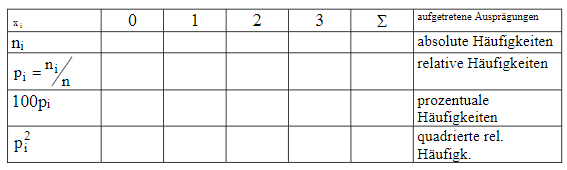
\includegraphics[width=\textwidth]{haeufigkeitstabelle-nominale-merkmale}
    \caption{Häufigkeitstabelle nominaler Merkmale}
    \label{fig:haeufigkeitstabelle-nominale-merkmale}
\end{figure}
\newline
Die Häufigkeitstabelle besteht aus $k$ Klassen bzw Kategorien. \newline
Aus der Tabelle kann man mehrere Sachen ablesen, die man ohnehin schon wusste:
\clm{Summe der absoluten Häufigkeiten}{}{Die absoluten Häufigkeiten, die der Tabelle ihren Namen geben, addierern sich zu $n$ (dem Stichprobenumfang)
\[\sum_{i=1}^{k} n_i = n\]
Beispiel: 3 Leute, davon 2 blond, einer dunkelhaarig. $2+1=3$.
}
\clm{Relative Häufigkeiten aus absoluten Häufigkeiten}{}{Dividiert man die absoluten Häufigkeiten durch $n$, erhält man die relativen Häufigkeiten. Damit kann man Stichproben mit verschiedenen Umfängen vergleichen. Die relativen Häufigkeiten addieren sich zu 1:
\[\frac{1}{n}\sum_{i=1}^{k} n_i = \sum_{i=1}^{k} p_i = 1\]
}
Um eine Idee von der Streuung der Daten zu bekommen, wird ein Maß eingeführt, welches man den \textbf{Index of Diversity} nennt:
\dfn{Index of Diversity}{
\[D = 1 - \sum_{i=1}^{k} p_i^2\]
Der Index of Diversity liegt in einem Wertebereich $0 \leq D < 1$.
Ein Wert von 0 bedeutet, dass alle Merkmalsausprägungen identisch sind (keine Vielfalt), während ein Wert nahe 1 auf eine hohe Vielfalt in der Verteilung der Merkmalsausprägungen hindeutet.
Es ist ratsam, den Wert $D$ nicht an 1, sondern an $1- k^{-1}$ zu vergleichen, weil k in den seltensten Fällen unendlich groß sein wird.
}

\subsection{Ordinalskalierte Merkmale}
Ordinalskalierte Werte sind Werte, die eine klare Hierarchie aufweisen, wobei die Abstände zwischen den Werten nicht gleich interpretiert werden können.
\begin{figure}[h]
    \centering
    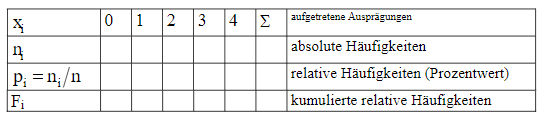
\includegraphics[width=\textwidth]{haeufigkeitstabelle-ordinale-merkmale}
    \caption{Häufigkeitstabelle ordinaler Merkmale}
    \label{fig:haeufigkeitstabelle-ordinale-merkmale}
\end{figure}
\newline
Das einzig Neue in dieser Tabelle (\ref{fig:haeufigkeitstabelle-ordinale-merkmale}) sind die \textbf{kumulierten relativen Häufigkeiten} (auch Summenhäufigkeiten).
Diese sind vor allem interessant, weil sie Vergleiche zwischen Stichproben unterschiedlicher Umfänge erlauben.
Dies ist aufgrund der eindeutigen Ordnung der Werte möglich.
\dfn{Kumulierte relative Häufigkeit}{
$F(x_i)$ stellt den Anteil der Werte dar, die höchstens die Merkmalsausprägung $x_i$ aufweisen.
\[F(x_i) = F_i = A(X \leq x_i) = \sum_{j=1}^{i} p_j \]
Üblicherweise wird die Summenhäufigkeit als Treppenfunktion dargestellt.
}
\newline
Übliche Kennwerte sind die \textbf{Quantile} (oder Prozentpunkte).
Die repräsentieren bestimmte Punkte einer Verteilung und teilen eben diese, basierend auf den kumulierten relativen Häufigkeiten, in gleich große Abschnitte ein. \newline
\dfn{Quantile}{
Quantile $X_w$ werden als die erste Merkmalsausprägung definiert, für welche die kumulierte relative Häfigkeit größer gleich $w$ ist.
\[F_i \geq w\]
Dies bedeutet, dass sie den Punkt in der Verteilung angeben, an dem mindestens ein bestimmter Prozentsatz $w$ der Daten erreicht oder überschritten wird.
}
\clm{Quartile}{}{
Zu den wichtigsten Quantilen gehören die Quartile.
Sie werden als $Q_i$ mit $i\in \{1,2,3\}$ angegeben.
Man spricht dann von dem ersten, zweiten oder dritten Quartil.
Die Quartile teilen die Rangwertreihe in 4 gleichmäßige Abschnitte auf und trennen bei 25\%, 50\% und 75\%.
}
Der \textbf{Median} ist ein bekanntes Beispiel für ein Quantil.
Er ist der Wert, bei dem die kumulierte relative Häufigkeit erstmals 50\% erreicht oder überschreitet.
Das bedeutet, dass 50\% der Daten kleiner oder gleich dem Median sind, während die anderen 50\% der Daten größer oder gleich dem Median sind.
Der Median ist somit $Q_2$ und berechnet sich als mittelster Wert der sortierten Liste, wenn die Anzahl der ungerade ist und als Mittelwert der beiden mittleren Werte, wenn die Anzahl gerade ist.


\subsection{Streuungsmaße}
\begin{itemize}
    \item Die \textbf{Spann- oder Streuweite} $R$ (wie Range) ist die Differenz zwischen den Extremwerten:
    \[R = x^{max} - x^{min}\]
    Die Streuweite wird üblicherweise zusammen mit dem Mittelwert angegeben, weil sie andernfalls nicht mehr aussagekräftigt wäre.
    \item Der \textbf{Interquartilsabstand} $IQA$ gibt den Bereich an, der von den mittleren 50\% der Werte bedeckt wird.
    \[IQA = Q_3 - Q_1\]
    \item Der \textbf{relative Quartilsabstand} berechnet sich aus dem Verhältnis von $IQA$ und $R$.
    Je näher diese Zahl an 1 ist, desto gestreuter ist die Verteilung.
    Je näher diese Zahl an 0 ist, desto konzentrierter ist die Verteilung.
    \[IQA_r = \frac{IQA}{R}\]
    \item Der \textbf{mittlere Quartilsabstand} $MQA$ wird als die Hälfte des $IQA$ definiert.
    \[MQA = \frac{IQA}{2} = \frac{Q_3 - Q_1}{2}\]
    Bei symmetrischen Verteilungen gilt entsprechend mit $Md$ als Median:
    \[MQA = \frac{Q_3 - Q_1}{2} = Q_3 - Md\]
\end{itemize}

\subsection{Intervallskalierte und diskret proportionalskalierte Merkmale}
Auch hier kann man den Median, Index of Diversity und bisher bekanntes berechnen.
Neu ist nachfolgend das arithmetische Mittel und die Standardabweichung.
\dfn{Arithmetisches Mittel (Durchschnitt)}{
Für den Durchschnitt, genauer: das arithmetische Mittel, wird die Summe aller Werte der Urliste berechnet und durch die Anzahl der summierten Werte addiert. Mathematisch ausgedrückt:
\[\overline{x}=\frac{1}{n} \sum_{j=1}^{n} x_j\]
Falls die Daten nur in Häufigkeitstabellen bzw relativen Häufigkeiten ($p_z$) mit $k$ Klassen gegeben sind, ändert sich die Formel wie folgt:
\begin{align*}
    \overline{x} &=\frac{1}{n} \sum_{j=1}^{n} x_j =\frac{1}{n} \sum_{z=1}^{k} x_z n_z =\sum_{z=1}^{k} x_z \frac{n_z}{n} \\
    &=\sum_{z=1}^{k} x_z p_z
\end{align*}
}

\clm{Symmstrie}{}{
Ist eine Verteilung symmetrisch, so ist der häufigste Wert in der Mitte, der Median auch und der Durchschnitt auch.
Deshalb gilt:
\[\overline{x} = \tilde{x} = x_D\]
Wobei $\overline{x}$ der Durchschnitt ist, $\tilde{x}$ der Median und $x_D$ der häufigste Wert ist.
}
Zu beachten ist außerdem, dass das arithmetische Mittel sehr empfindlich gegenüber Ausreißern in den Daten ist.
Eine eigentlich sehr konzentrierte Verteilung mit einzelnen Werten weit ab vom Rest, kann den Durchschnitt erheblich beeinflussen.
So wäre der Durchschnitt von $X_1 = \{1,2,3,4,4,3,2,1\}$ gleich $2.5$ ist, während der Durchschnitt von $X_2 = \{1,2,3,4,4,3,2,25\}$ gleich $5.5$ ist.
Hieran sieht man deutlich, dass ein solcher Ausreißer den Durchschnitt in seiner Aussagekraft deutlich mindert.

\clm{Summe der Abweichungen vom arithmetischen Mittel ist immer 0}{}{
Gegeben ist eine Urliste von Werten $X$ mit Mächtigkeit $n$ und dem zugehörigen arithmetischen Mittel $\overline{x}$.
Es gilt immer:
    \[\sum_{j=1}^{n}(x_j - \overline{x}) = 0 \]
Im gleichen Zuge die \textbf{Abweichung vom Durchschnitt} für die j-te Ausprägung wie folgt definiert:
\[x^\ast = x_j - \overline{x}\]
Verdeutlicht an einem Beispiel mit $X = \{1,2,3\}$ und entsprechend $\overline{x} = 2$:
\begin{align*}
    Abweichung &= \sum_{j=1}^{n}(x_j - \overline{x}) = \sum_{j=1}^{3}(x_j - \overline{2}) \\
    &= (1-2) + (2-2) + (3-2) \\
    &= -1 + 0 + 1 \\
    &= 0
\end{align*}
}
Weil mit dieser Darstellung der Abweichung vom Durchschnitt nicht gut zu arbeiten ist (und sie maximal Rechenfehler aufzeigen kann).
Diese Tatsache zeigt lediglich, dass das arithmetische Mittel einen Gleichgewichtspunkt in der Verteilung der Urliste darstellt.
Es gibt jedoch Möglichkeiten, die Abweichung vom Durchschnitt so zu modifizieren, dass sie ein aussagekräftiger Indikator im Messen von Abweichungen werden kann.
\dfn{Mittlere quadratische Abweichung}{
Es wird $d^2$ als mittlere quadratische Abweichung definiert, in dem die Abweichung vom Durchschnitt quadriert wird und man den Durchschnitt der quadrierten Abweichungen berechnet. $x_j^\ast$ stellt in diesem Fall die Abweichung vom Durchschnitt für die j-te Ausprägung dar:
\[d^2 = \frac{1}{n} \sum_{j=1}^{n} x_j^{\ast 2} = \frac{1}{n} \sum_{j=1}^{n}(x_j -\overline{x})^2 \]
}
Aus der mittleren quadratischen Abweichung lässt sich anschließend die Stichprobenvarianz berechnen.
\dfn{Stichprobenvarianz}{
Die Stichprobenvarianz $s^2$ wird wie folgt berechnet:
\[s^2 = \frac{1}{n-1} \sum_{j=1}^{n} x_j^{\ast 2} = \frac{1}{n-1} \sum_{j=1}^{n}(x_j -\overline{x})^2\]
Der offensichtlich einzige Unterschied zu $d^2$ liegt darin, dass die Summe keinen Faktor mehr von $n^{-1}$ aufweist, sondern einen Faktor von $(n-1)^{-1}$.
Entsprechend lässt sich die Stichprobenvarianz auch wie folgt beschreiben:
\[s^2 = \frac{n}{n-1}\cdot d^2\]
}
Mit der definierten Stichprobenvarianz lässt sich das bekannte Abweichungsmaß der \textbf{Stichprobenstandardabweichung} bestimmen.
\dfn{Stichprobenstandardabweichung (Standardabweichung)}{
Die Stichprobenstandardabweichung $s$ ist wie folgt definiert:
\[s = \sqrt{s^2} = \sqrt{\frac{1}{n-1} \sum_{j=1}^{n}(x_j -\overline{x})^2} = \sqrt{\frac{n}{n-1}\cdot d^2}\]
Man kann bei $s$ annehmen, dass es in den sleben Einheiten ausgedrückt wird, wie die Daten selber.
Die Standardabweichung stellt die durchschnittliche Abweichung aller Werte von dem arithmetischen Mittel dar.
}
\clm{Mittleres Schwankungsintervall}{}{
Am aussagekräftigsten ist die Angabe des mittleren Schwankungintervalls:
\[\overline{x} \pm s = [\overline{x} - s, \overline{x} + s]\]
Je mehr sich die Grenzen dieses Intervalls von den Grenzen des Definitionsbereichs der Urliste absetzt, desto weniger streut die Verteilung.
}
Die praktische Vorgehensweise zur Berechnung von $s$ benötigt zusätzlich den \textbf{Durchschnitt der Quadrate} der Merkmalsausprägungen:
\[\overline{x^2} = \frac{1}{n} \sum_{j=1}^{n} x_j^2\]
um $d^2$ wie folgt zu definieren:
\[d^2 = \overline{x^2} - \overline{x}^2\]
\\
\dfn{Variationskoeffizient}{
Der Variationskoeffzient $v$ ist ein Maß, welches ein Vergleich zwischen zwei Verteilungen schaffen kann.
Er gibt an, wie viele \% des Arithmetischen Mittels von der Standardabweichung ausgemacht werden und wird wie folgt berechnet:
\[v = \frac{s}{\overline{x}}\]
$v$ kann $<1$ oder $>1$ sein, allerdings niemals negativ.
Ist $v$ kleiner als $1$, so ist die Standardabweichung kleiner als der Mittelwert ist und die Daten relativ eng um den Mittelwert herum verteilt sind.
Umso weiter $v$ gegen $0$ geht, desto enger liegen die Werte um $\overline{x}$ herum.
Gegenteilig sind die Werte weit um $\overline{x}$ herum gestreut, wenn $v$ größer als 1 sein sollte.
Der Variationskoeffizient sollte also genutzt werden, um zwei Verteilungen auf ihre Streuung hin zu vergleichen.
}
\ex{Beispiel zum Variationskoeffizienten}{
Gegeben sind die beiden Datensätze $X_1 = \{1,2,2,2,3,4\}$ und $X_2 = \{-20,1,1,1,40,400\}$.
Für diese wird nun jeweils der Variationskoeffizient berechnet: \newline
Datensatz 1:
\begin{itemize}
    \item $\overline{x} = 2.33$
    \item $s = 1.03$
    \item $v = 1.03\cdot 2.33^{-1} = 0.44$
\end{itemize}
Datensatz 2:
\begin{itemize}
    \item $\overline{x} = 70.5$
    \item $s = 146.26$
    \item $v = 146.26\cdot 70.5^{-1} = 2.07$
\end{itemize}
Hier ist deutlich zu sehen, was das Betrachten der Datensätze schon vermuten lässt: Datensatz 2 ist deutlich weiter gestreut, als Datensatz 1.
Die Streuung von Datensatz 1 ist sogar als recht eng zu beurteilen, weil $v$ eher gegen 0, als gegen 1 geht.
}
